\chapter{Brain Imaging Data Structure (BIDS)}
\label{chapter:group_study}

\epigraph{\small\itshape ``Data! data! data! I can't make bricks without clay.''}
{\small\textit{---Sherlock Holmes}}

\begin{figure}[ht!]
\centering
\begingroup
\etocstandardlines
%\renewcommand{\etocbkgcolorcmd}{\color{lightgray}}
\renewcommand{\etocbelowtocskip}{0pt\relax}
\fboxsep1ex
\etocframedstyle [1]{\fbox{\makebox[.4\linewidth]{\etocfontminusone
Contents}}}
\localtableofcontents
\endgroup
\end{figure}

\clearpage

\section{Context}
While data sharing in neuroscience is on the rise, the amount of data reuse is still limited. For instance, since the release of the Human Connectome Project (HCP)~\citep{larson2013adding} MEG data in 2013, there have been only one or two documented cases~\citep{jas2017autoreject} of reusing the data. Even in these cases, the effort has mostly been to reproduce rather than test new hypotheses. This clearly represents a gap between the ideal of data sharing and the consequences in practice. 

% Clearly, sharing data is not a panacea as the tools, skills and resources to process such large datasets is currently missing in typical laboratories. Perhaps the most important roadblock is standardization of metadata.

\subsection{The need for standards}

\begin{figure}[htb]
\begin{center}
   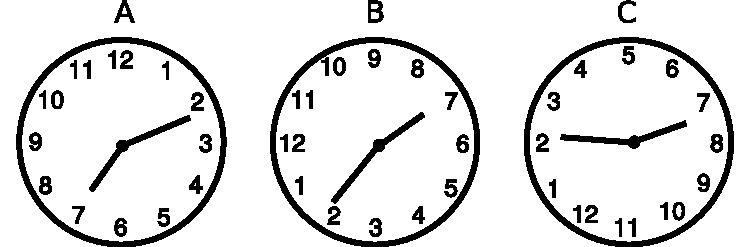
\includegraphics[width=0.7\linewidth]{figures/clock.pdf}
\end{center}
   \caption[Standards in clocks]{Standards in clock design. The time is 07:11 (A) Modern standard, read clockwise and 12 o' clock is at North (B) Anticlockwise and 9 o' clock at North (C) Read clockwise but 5 o' clock is at North. Adapted from \cite{norman2013design}.}
   \label{fig:clock_standards}
\end{figure}
% Data sharing is clearly not productive if the data is not easily  \emph{reusable} in the same way that uncommented and spaghetti code cannot be reused even if it is shared publicly. 
Neuroimaging experiments are often complicated involving different paradigms (auditory, visual, somatosensory \emph{etc.}), different acquisition parameters (sampling frequency, number of sensors and their location, measurement device \emph{etc.}), and population parameters: subject's gender, age \emph{etc.} Obviously, this metadata is necessary information to reanalyze the data.   

Unfortunately, there has been historically, a lack of consensus amongst different labs and industrial manufacturer's as to what constitutes useful metadata. This points to the need for establishing standards. While on a superficial glance, this may appear to be unnecessary bureaucratic red tape, the need for standards can be appreciated by considering the simple wall clocks in Figure~\ref{fig:clock_standards}.

The wall clock is recognized as an everyday object that is perhaps far simpler than most complex neuroimaging experiments. Even then, there are two degrees of freedom even to this simple device: the direction of motion of the hands, and the anchor point for the 12 o' clock. While all three clocks in the figure can still be readable, it is far more convenient to establish a standard. The upfront cost in conforming to the standard is more than made up by the efficiencies achieved as a result of it.

Apart from the metadata that is stored with the data, the data itself is stored amongst one of 10--20 different file formats and at different stages of processing. While there have been some efforts previously to standardize data structures~\citep{gibson2009minimum, grewe2011bottom, stoewer2013singlefile, teeters2015neurodata, bigdely2016preparing}, it has not gained wide acceptability. Designing a new standard is tricky as it requires gaining a community consensus. At the same time it must strike the right balance between rigidity for efficiency and flexibility for adapting to future technologies. 

\subsection{The standard}
The BIDS format is indeed designed with these considerations in mind. The standard involves a hierarchy of folders to describe the imaging technology used, the name of the subject, and the date of the experiment. At each level of hierarchy, files are accompanied by sidecar \code{json} files describing the metadata. These files follow an inheritance principle, that is, a field described in a \code{json} file in a higher level of the hierarchy will be automatically propagated downstream. The main BIDS specification is accompanied by extension specifications which describe specific aspects of describe certain file types. The BIDS consortium is also providing a growing ecosystem of tools to convert datasets into BIDS compatible format as well as to validate data to conform to the standard. 

The development of these standards is going to enable building large databases of neural recordings. In the future, we can envision being able to open a website and query or search through such data by different experimental paradigms or other metadata.

\noindent\fcolorbox{white}{lightgray}{%
\begin{minipage}{\dimexpr\textwidth-2\fboxrule-2\fboxsep\relax}
\begin{itemize}[align=left, leftmargin=10pt, labelwidth=5pt, labelindent=10pt, itemsep=5pt, topsep=5pt]
  \item[] Section~\ref{sec:BIDS-MEG} was published in:
  \item \bibentry{galan2017meg}
\end{itemize}
\end{minipage}}%

\section{Introduction}
The Brain Imaging Data Structure (BIDS) is an emerging standard for the organization of neuroimaging data1. The significance of BIDS is timely: there is increasing availability of open neuroimaging data resources, and strong interest in aggregating large, heterogeneous datasets to harness machine learning techniques and address a new range of scientific questions, with greater statistical power. A single neuroimaging study by itself can represent a large and intricate volume of data, with multiple protocols and modalities, and several categories of participants possibly enrolled in repeated sessions. These aspects are challenging to data organization, harmonization and sharing. The situation is aggravated by the lack of a unique neuroscience standard for digital data across, and sometimes within, modalities such as electrophysiology. Consequently, present data management practices are often based on solutions that do not generalize between labs, or even between persons within the same group. This leads to suboptimal usage of human (time lost retrieving data), infrastructure (data storage space) and financial (limited longevity and value of disorganized data after first publication) resources. Poor or lacking data management strategies also negatively affects the reproducibility of results, even within the lab where the data were collected. 
BIDS is a standard to describe the organization of magnetic resonance imaging (MRI) data. It is based on a simple, hierarchical folder structure, with key study parameters documented in text-based metadata files. One benefit is the handling of multiple MRI data sequences, with minimal curation overheads, which reduces the possibility of data-handling errors. An important secondary outcome is the facilitation of interoperability between tools for data analytics, provided that software and pipelines adopt BIDS for data inputs. 

We describe here a key extension of BIDS to electrophysiology data. The technical sophistication of MEG makes it the most challenging electrophysiology data type for standardization2. For this reason, BIDS-MEG can readily be generalized to electroencephalography, multiunit recordings, and local field potentials. Further to strengthening and rationalizing data management in MEG labs, BIDS-MEG provides a common structure to present and future large MEG open-data repositories3,4,5. The absence of unique data file format in MEG is compensated by BIDS-MEG’s standard data organization: the sharing and processing of large and complex data hierarchies is simplified, and made compatible and reproducible across tools for data analytics. 

To derive the BIDS-MEG specifications, we have combined perspectives from investigators, technical support staff and data managers. We also involved the expertise of leading academic software developers for MEG science6, including Brainstorm7, FieldTrip8, MNE9, and SPM10. The proposed BIDS-MEG specifications are presently compatible with these software applications and toolboxes.

\section{Technical specification}
\label{sec:BIDS-MEG}

\begin{figure}[htb!]
\begin{center}
   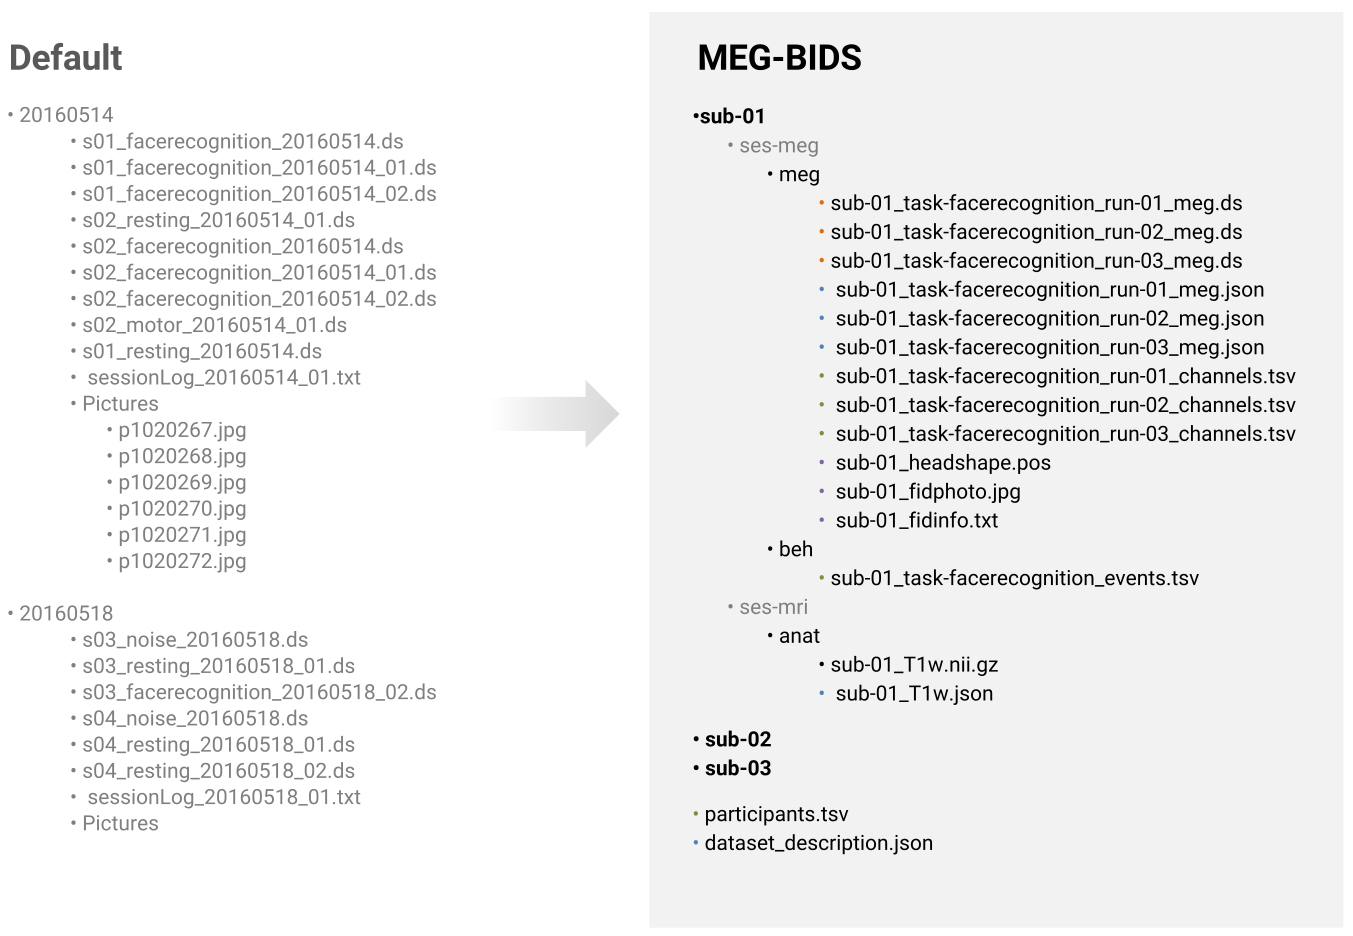
\includegraphics[width=\linewidth]{figures/bids_organization.png}
\end{center}
   \caption[BIDS-MEG data organization scheme.]{BIDS-MEG data organization scheme: Left: a typical default data organization scheme where folder are organized by date of session and contain different runs for a given participant in a study. Right: BIDS-MEG organizes data per study, then participant (subject), followed by modality, then sessions and eventually, runs. Note the sidecar files that are present at all level the data hierarchy, and document conveniently the metadata contents.}
   \label{fig:BIDS-MEG-organization}
\end{figure}


\begin{sidewaysfigure}[htb!]
\begin{center}
   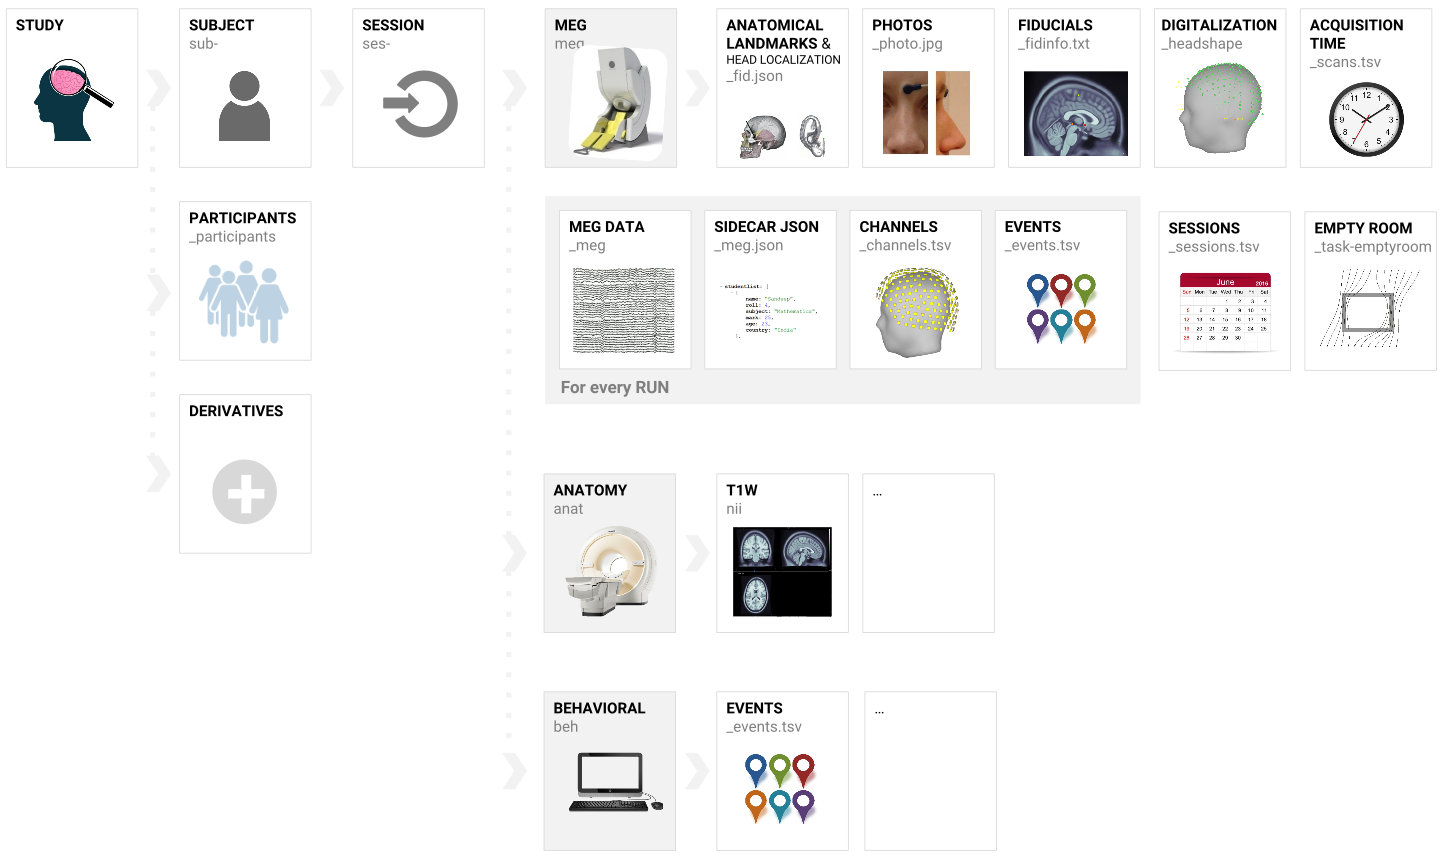
\includegraphics[width=\linewidth]{figures/bids_structure.png}
\end{center}
   \caption[BIDS-MEG general overview]{ BIDS-MEG general overview}
   \label{fig:BIDS-MEG-overview}
\end{sidewaysfigure}

\begin{sidewaysfigure}[htb!]
\begin{center}
   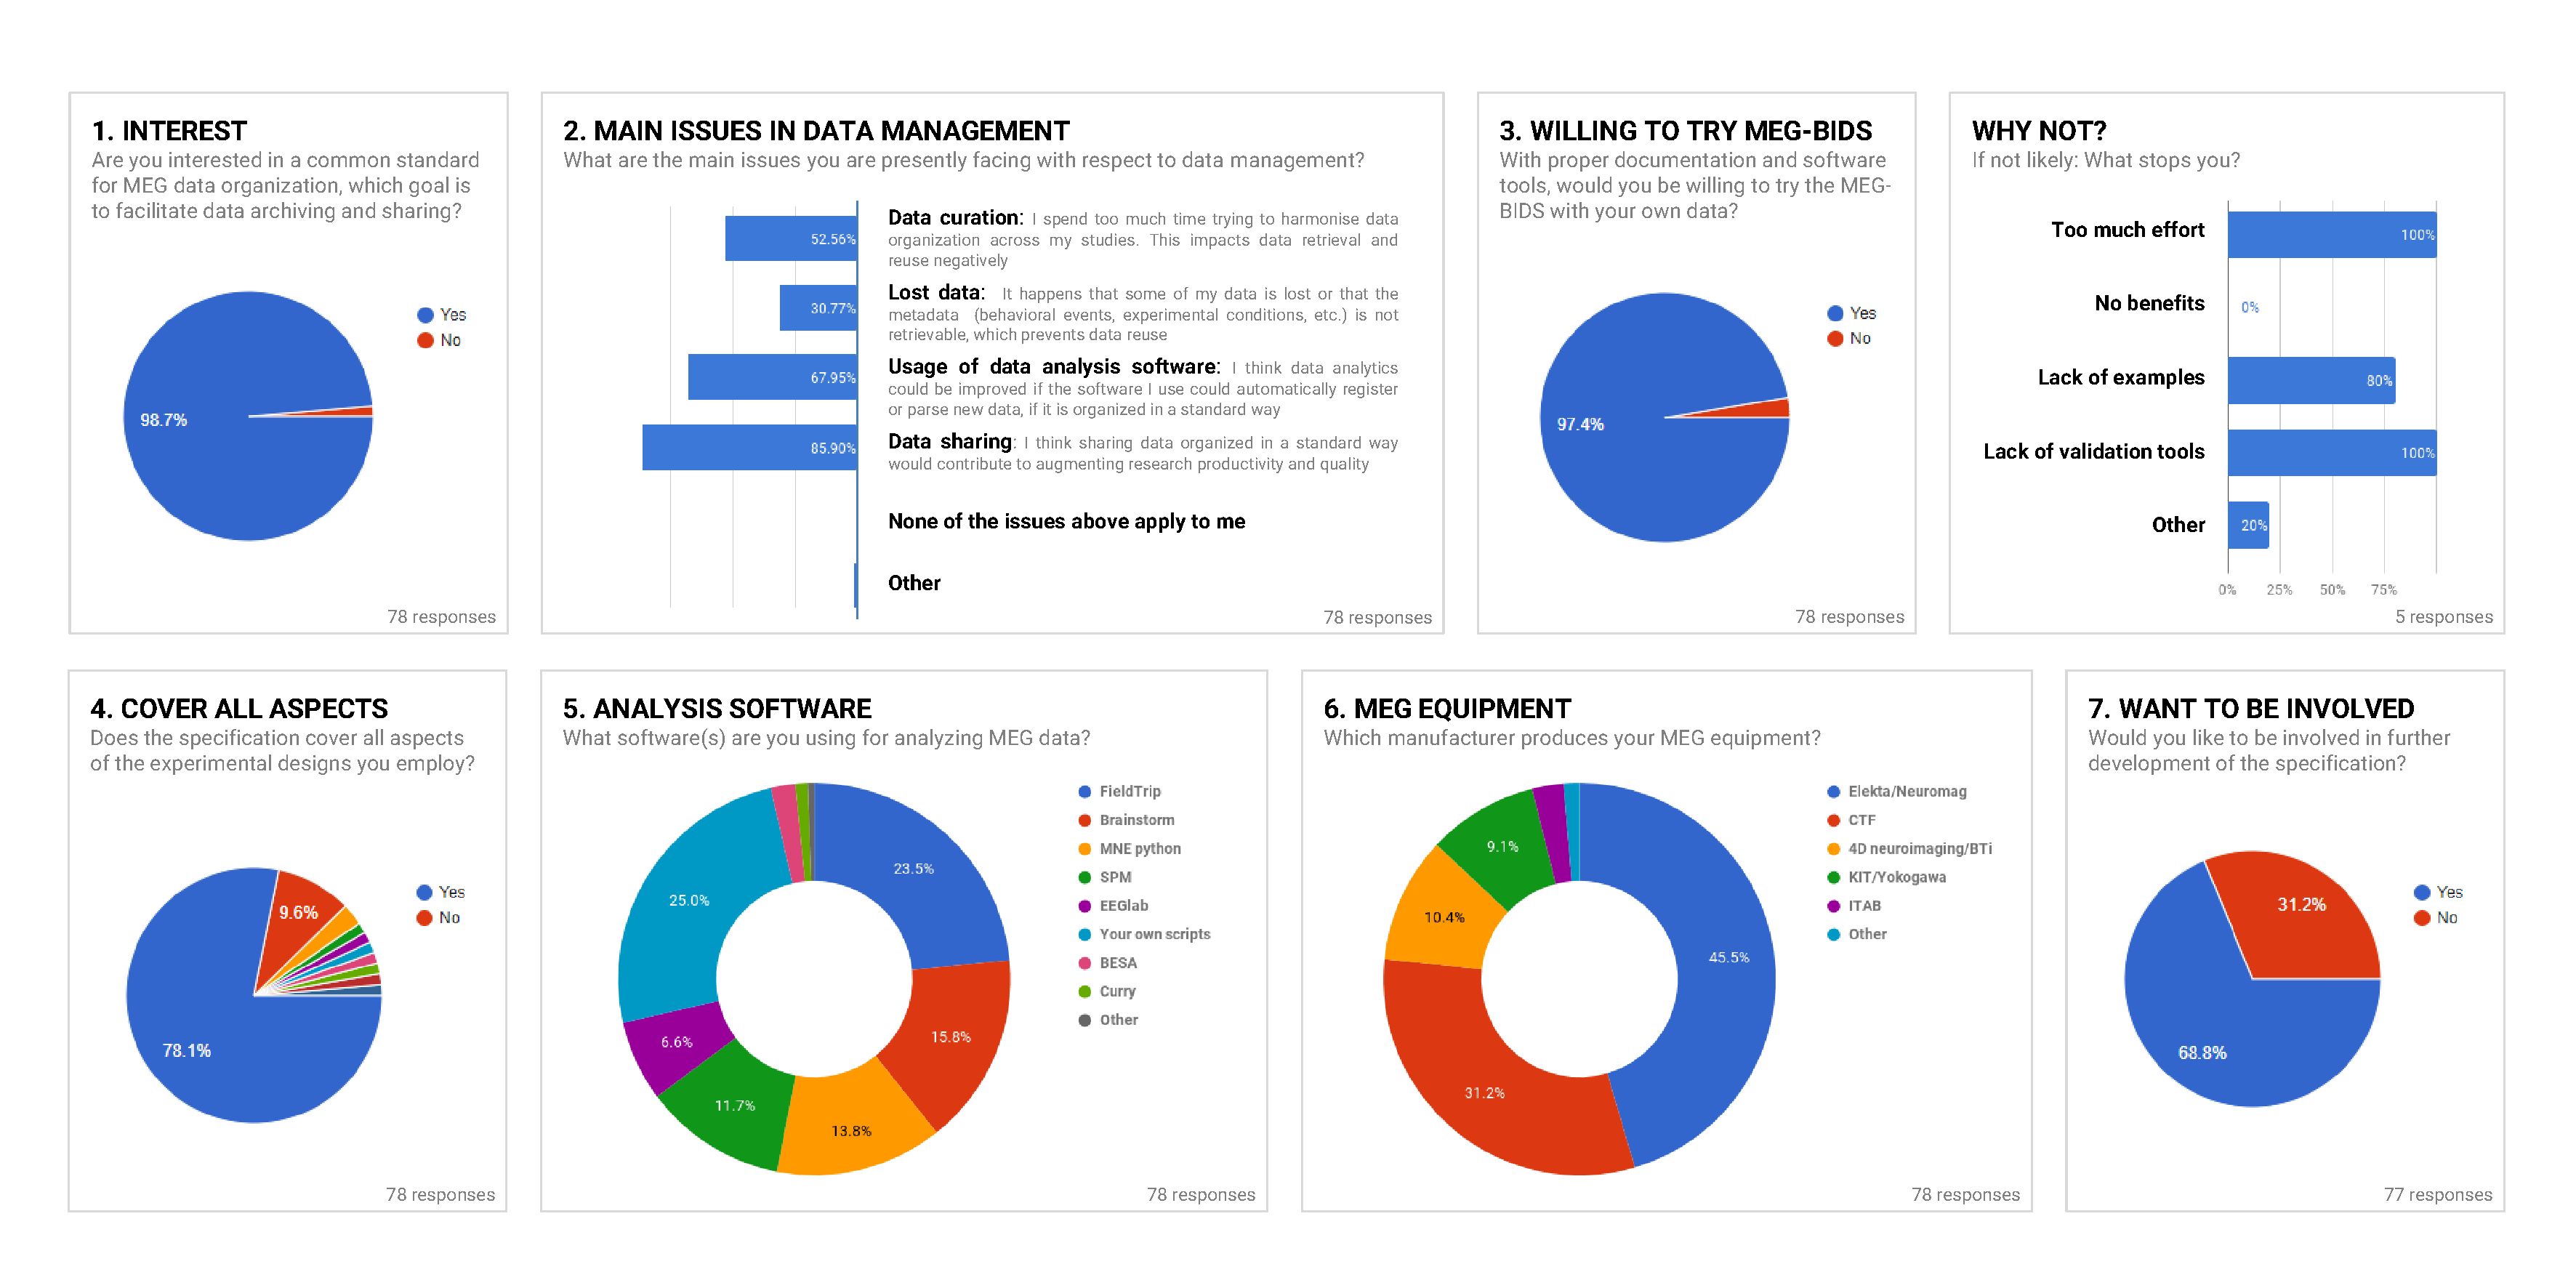
\includegraphics[width=\linewidth]{figures/MEG-BIDS_poll_results_figure.pdf}
\end{center}
   \caption[Results from the BIDS-MEG poll.]{Results from the BIDS-MEG poll}
   \label{fig:BIDS-MEG-poll}
\end{sidewaysfigure}

The BIDS-MEG fields and data organization were defined, bearing in mind best-practice guidelines for conducting MEG research~\citep{gross2013good}. The initiative fostered contributions from multiple MEG experts, with a face-to-face discussion at the 2016 International Conference on Biomagnetism, where the first incarnation of BIDS-MEG was introduced~\citep{niso2016megbids}. The first set of feedback comments and the minutes from further group discussions are publicly available
(\url{https://groups.google.com/d/msg/bids-discussion/xTHBsGhu0hk/MN25xbxRBwAJ}).

A first version of the present manuscript was shared via the preprint server bioRxiv, from where more comments stemming from the community were collected and considered for improvement of BIDS-MEG. A poll survey to probe the interest of the concerned community was also conducted (see main results on Figure~\ref{fig:BIDS-MEG-poll}).

BIDS-MEG builds on the BIDS hierarchical data structure. For instance data descriptors such as subject, session, technique, run are BIDS notions that were re-used in BIDS-MEG. Similarly, the simple although extensively used human and machine readable file formats (JavaScript Object Notation [JSON], and Tab Separated Value [TSV] text files) that contributed to the versatility and practicality of documenting metadata elements in BIDS, were expanded with BIDS-MEG. BIDS-MEG employs a straightforward terminology, cautiously defined in line with the general BIDS specifications, although adapted to the unique requirements of MEG.  For further reference, the BIDS-MEG specifications are detailed in an open-access online document:
\url{https://docs.google.com/document/d/1FWex_kSPWVh_f4rKgd5rxJmxlboAPtQlmBc1gyZlRZM)}

The terms used refer to notions that were defined by reaching a consensus amongst the BIDS-MEG contributors and the MEG community. For example, ‘Subject’ refers to the scanned participant. Note that from a technical standpoint, MEG is not a scanning technique. Yet, we used this terminology for convenience, affinity with other neuroimaging modalities, and to reflect the language used in most MEG labs. A ‘Session’ defines a non-intermittent period of time during which the subject is in the scanner.  A ‘Run’ is a period of time during which empty-room (for noise characterization) or brain activity is recorded continuously, with no interruptions. It is typical with MEG that a session consists of multiple runs: task instructions can change and/or participants can take a break between runs. The notion of ‘Task’ refers to the instructions (and corresponding stimulus material) that are performed by the participant. ‘Responses’ is a feature to indicate the recorded behaviour of the subject in relation to the task.

As with the general BIDS specifications~\citep{gorgolewski2016brain}, BIDS-MEG file names are constituted by a series of key-value pairs, with multiple possible file types. Some  typological aspects are mandatory, while others remain optional, although required to abide to the BIDS guidelines. BIDS-MEG can therefore register data of any kind, including but not limited to task-based, resting-state, and empty-room MEG recordings (e.g., for noise estimation purposes). We emphasize that all of the above notions apply also to EEG, and all modalities of electrophysiology, for which BIDS-MEG serves as template for standardization.  

There is no common, open or standard file format in MEG, equivalent to DICOM or NIfTI in MRI. MEG systems manufacturers (CTF, Elekta/Neuromag, BTi/4D Neuroimaging, KIT/Yokogawa/Ricoh, Tristan Technologies, ITAB, KRISS/Compumedics Neuroscan, York Instruments) all cater a vendor-specific format. With BIDS-MEG, unprocessed (raw) data is stored in the native file format (see Discussion for further consideration of common MEG format initiatives) and users can still rely on their preferred data analysis application, possibly provided by the MEG vendor, to browse and read in the MEG file contents. Software can also extract meta information elements from the raw data files. They concern e.g., data collection parameters and other study descriptors, which are eventually transcribed into sidecar JSON files by said BIDS-MEG compatible applications. One major benefit of metadata extraction is the facilitation of subsequent data searches and indexation, without the handling and repeated parsing of large raw data files. Additional relevant files can be included alongside the MEG raw data: some propositions are detailed in the online specifications.

For a given investigator or research group, BIDS-MEG describes a hierarchical structure that descends from a ‘Study’ folder. Multiple ‘Subject’ subfolders contain the data from the participants enrolled. They are arranged by ‘Session’, each session subfolder containing ‘Run’ folders and eventually, data and metadata files. 

The ‘Run’ folder includes a variety of files: MEG recording files in native format, a sidecar JSON document (\code{*\_meg.json}), a channel description table (\code{*\_channel.tsv}), and other general BIDS files, such as task events tables (\code{*\_events.tsv}) that are likely to be specific of each run. ‘Session’ specific files include the coordinates of anatomical landmarks and head-localization coils stored in a JSON document (\code{*\_fid.json}), optional photographs of the anatomical landmarks and/or head localization coils  (\code{*\_photo.jpg}), fiducials information (\code{*\_fidinfo.txt}), 3-D scalp digitalization files (\code{*\_headshape.<manufacturer\_specific\_format>}) and acquisition times (\code{scans.tsv}). The ‘Subject’ and ‘Study’ specific files are inherited directly from the general BIDS specifications (e.g., participants.tsv). Note that in case of conflict between fields of different runs/sessions, it the inheritance principle should be applied: the description file closer to the data prevails (see Section ‘3.5 The Inheritance Principle’ of the BIDS specifications~\citep{gorgolewski2016brain}.

One issue that required special attention was the multiplicity of coordinate systems and units between MEG systems. To impose a unique coordinate system for BIDS based on the subjects’ brain anatomy (e.g., MNI coordinates or equivalent) was an appealing solution, which however would lack generalizability in the MEG practice. MEG data can be collected without anatomical information, such as empty-room noise recordings, which are important to optimal source modeling~\citep{gross-etal:13}. BIDS-MEG therefore associates all recordings with a coordinate file defined according to the MEG system used. Again, BIDS-MEG compatible software can read and interpret this information properly.

Akin to MRI, we anticipate that the systematic data organization enabled by BIDS-MEG will be supported by an increasing number of neuroimaging tools, and that more shared data repositories will be organized accordingly. The straightforward design of BIDS-MEG makes it an interoperable common exchange format for transferring data between investigators and community repositories e.g., OMEGA~\citep{niso2016omega} and OpenfMRI~\citep{poldrack2017openfmri}. It also facilitates multimodal integration (between MRI, fMRI, MEG, etc), as the data from multiple modalities follow the same organization scheme.

\section{Open BIDS-MEG datasets}
We provide four different publically-available datasets in BIDS-MEG format ($\sim$200GB). They are freely available for download from the International Neuroinformatics Coordinating Facility (INCF)’s  GitHub: \url{https://github.com/INCF/BIDS-examples/tree/bep008_meg}

The BIDS-MEG sample data release includes: 

\paragraph{OMEGA Resting-State samples:} Five minutes of eyes-open, resting-state MEG data is available for 5 subjects from The Open MEG Archive (OMEGA)4. The data are available from the Brainstorm Tutorial: MEG resting state \& OMEGA database. The first release of data in BIDS-MEG format ($\sim$10.5GB) available here: 
\url{https://box.bic.mni.mcgill.ca/s/omega?path=\%2FContributions
\%20(in\%20BIDS\%20format)\%2Fsample_BIDS_omega} (access to these datasets require registration to OMEGA, \url{https://www.mcgill.ca/bic/omega-registration}).

\paragraph{Brainstorm Auditory Example dataset:} Brainstorm Auditory tutorial dataset8 (~2.3GB):
\url{https://box.bic.mni.mcgill.ca/s/omega?
path=\%2FContributions\%20(in\%20BIDS\%20format)
\%2Fsample_BIDS_auditory} (released in Public Domain; includes defaced anatomical T1 of participant, access to these datasets require registration to Brainstorm, \url{http://neuroimage.usc.edu/bst/register.php}). 

\paragraph{MNE Sample data:} Sample data with visual and auditory stimuli described in11:
\url{https://drive.google.com/drive/folders/0B_sb8NJ9KsLUQ3BMS0dxZW5nSHM?usp=sharing} (released in Public Domain; includes anatomical T1 of participant as well as flash MRI sequences). 

\paragraph{OpenfMRI study ds000117:} A multi-subject, multi-modal human neuroimaging dataset of 19 subjects participating in a visual task16 ($\sim$178GB): \url{https://openfmri.org/dataset/ds000117/}. This dataset is used in one of the SPM tutorials, for training purposes:
\url{http://www.fil.ion.ucl.ac.uk/spm/doc/manual.pdf#Chap:data:multimodal}

\subsection{Software}
Widely used MEG software packages have already added functionality to support BIDS-MEG:

\paragraph{Brainstorm}\citep{tadel2011brainstorm}: Brainstorm is an application with rich graphical-user interactions and analytic pipeline designs for MEG, EEG, NIRS, and electrophysiology recordings. BIDS-formatted MEG/EEG datasets can be imported automatically into the Brainstorm database, as described in the OMEGA tutorial: \url{http://neuroimage.usc.edu/brainstorm/Tutorials/RestingOmega}

\paragraph{FieldTrip}\citep{oostenveld2010fieldtrip}: FieldTrip is an open-source MATLAB toolbox for the analysis of MEG, EEG, and other electrophysiological data. Like most other tools listed herewith, FieldTrip can  implement full analysis pipelines, starting from coregistration, preprocessing, time- and spectral analysis, source reconstruction, connectivity and statistics. Among others, FieldTrip has been used for the MEG part of the Human Connectome Project. Since a FieldTrip analysis pipeline is represented as a MATLAB script, its application on BIDS structured data implies that the BIDS details are represented in the analysis scripts that users write. 

\paragraph{MNE}\citep{gramfort2013meg, mne}: MNE (http://martinos.org/mne), whose name stems from its capability to compute cortically-constrained minimum-norm current estimates from M/EEG data. It is a software package that provides comprehensive analysis tools and workflows including preprocessing (Maxwell filtering, ICA, signal space projectors), source estimation (eg. using MNE, beamformers or mixed-norm sparse solvers), time-frequency analysis, statistical analysis including multivariate decoding, and several methods to estimate functional connectivity between distributed brain regions. The core of MNE is written in Python and is distributed under the permissive BSD Licence. MNE will use the BIDS data structure to distribute all its tutorial datasets and the documented analysis scripts. MNE provides Python code to read and write files in BIDS compatible format, as well as summary reports automatically generated via the MNE report command. A preliminary version is available at \url{https://github.com/mne-tools/mne-bids}. 

\paragraph{SPM}\citep{litvak2011eeg}: SPM (\url{http://www.fil.ion.ucl.ac.uk/spm}) is a free and open source software written in MATLAB where many widely used methods for the analysis of PET, fMRI and for computational neuroanatomy have been originally developed and implemented. More recently SPM has been extended to perform M/EEG analyses, including topological inference for neurophysiological data, empirical Bayesian framework for source reconstruction and Dynamic Causal Modeling (DCM), an approach combining neural modeling with data analysis. SPM~\citep{litvak2011eeg} includes a library, spm\_BIDS.m, to parse and query BIDS-formatted datasets, as well as low-level functions to read/write JSON and TSV metadata files. A complete pipeline for the analysis of a group MEG dataset in BIDS format is presented in preparation.

Other BIDS-MEG tools

Another set of tools have been developed to generate sidecar BIDS-MEG JSON files, and assist researchers in their evaluation  and adoption of the standard. These Python scripts are publically available:  \url{https://github.com/INCF/pybids}.

For a more detailed description of the BIDS-MEG specification, example datasets, resources and feedback, please visit \url{http://bids.neuroimaging.io}.

\section{Discussion}
Although BIDS-MEG is a proposal to establish a standard framework for the organization of electrophysiology data, it does not impose the standardization of the data file format per se. Some initiatives are aiming towards the definition of a new common binary file format for electrophysiology (MNE python group). Akin to DICOM in MRI, one single file format would beneficial, when considering the diversity of native raw file formats in electrophysiology. Yet, MEG data volumes are typically very large (several GBs), hence their duplication into a standard format may be unimpractical. Our position is rather to promote BIDS-MEG and ascertain that tools for data analytics continue to be equipped with the necessary readers for all existing vendor formats. We believe the capacity of BIDS-MEG to organise data without requiring a common data format is actually a strength: the standard is flexible in the sense that any data parameters can be extracted and stored as metadata in sidecar json files at the time of creating a new data entry, regardless of the file format for the raw data. Therefore, any new data format for electrophysiology, including emerging standards, is by construction compatible with BIDS-MEG.

Along the same lines, special attention was given to the handling of the various  coordinate systems used by the different MEG vendors and toolboxes. BIDS-MEG is also flexible in that respect, as long as the conventions used are characterized and documented in the \code{*\_fid.json} file. The coordinate systems presently handled by BIDS-MEG are detailed in the Specification document. The coordinate systems used for MEG and EEG sensors, MRI volumes, locations of fiducials, anatomical landmarks and digitized head points, need to be described following this principle, as some are likely to be different.

We aim at extending BIDS-MEG further towards the handling of processed data, which for now and akin to MRI-BIDS, are simply stored in a data Derivatives folder.

BIDS-MEG represents a significant effort towards a common standard for MEG. We anticipate that the BIDS-MEG software ecosystem and the variety of publicly available BIDS-MEG datasets will grow and incentivize the research community towards adoption. 
